\section{Câu 13}
Cho mạch điện như ở Hình 8a. OPAMP được cấp nguồn có $V_{OH}=3.3V$, $V_{OL}=-3V$.
Các điện trở được chọn $R_1=2K$, $R_2=3K$, $R_3=4K$, $R_4=6K$.\\
Cho dạng sóng Vi(t) như ở Hình 8b. Vẽ dạng sóng ngõ ra Vo trong các trường hợp sau:\\
a. $V_1=2V$, $V_{m1}=2V$, $V_{m2}=-3V$\\
b. $V_1=4V$, $V_{m1}=1V$, $V_{m2}=-3V$
\begin{figure}[H]
	\centering
	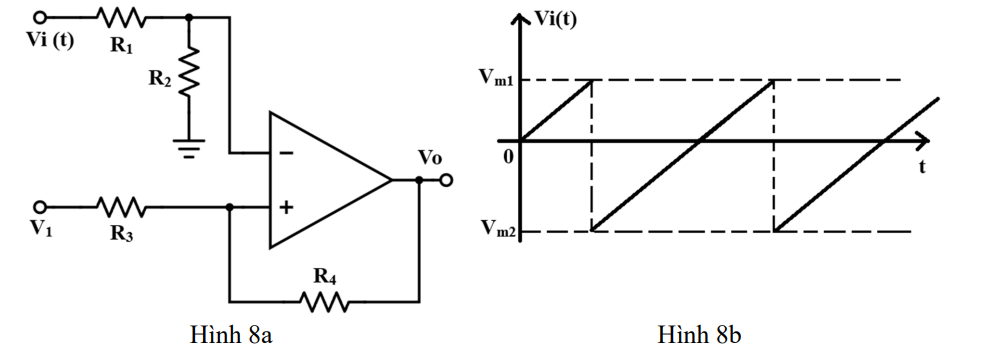
\includegraphics[scale=0.9]{image/C13_De.png}
\end{figure}
\begin{center}
\textbf{Bài giải}
\end{center}
a. Giả sử OPAMP lý tưởng:\\
Ta có:
\[
\left\{
\begin{aligned}
V^- &= \dfrac{R_2}{R_1+R_2}V_i \\
V^+ &= \dfrac{\dfrac{V_1}{R_3} + \dfrac{V_o}{R_2}}{\dfrac{1}{R_3} + \dfrac{1}{R_4}} = \dfrac{3}{5}V_1 +\dfrac{2}{5}V_o
\end{aligned}
\right.
\]

\[
\begin{aligned}
&\text{Giả sử }& V_o = V_{OH} &\qquad\rightarrow\qquad V^+ = \dfrac{3}{5}\cdot2 + \dfrac{2}{5}\cdot3.3 \quad;\quad V^- = 0.6V_i \\
&\text{Để }& V_o = V_{OL} &\qquad\rightarrow\qquad V^+ < V^- \quad\rightarrow\quad \boxed{V_i>4.2V}\\
&\rightarrow& V_o = V_{OL} &\qquad\rightarrow\qquad V^+ = \dfrac{3}{5}\cdot2 + \dfrac{2}{5}\cdot-3 \quad;\quad V^- = 0.6V_i \\
&\text{Để }& V_o = V_{OH} &\qquad\rightarrow\qquad V^+ > V^- \quad\rightarrow\quad \boxed{V_i<0V}\\
\end{aligned}
\]\\
Tại t=0 đến khi $V_i(t)=0$ nằm trong khoảng Deadband của OPAMP. Vì thế tùy vào trạng thái ban đầu sẽ cho ra ngõ ra khác nhau.
Sau khi $V_i(t)<0$ thì $V_o = V_{OH}$ và $V_i$ luôn bé hơn 4.2V nên không thể cho $V_o=V_{OL}$. Vì thế nên $V_o$ từ đó luôn bằng $V_{OH}$
\begin{figure}[H]
	\centering
	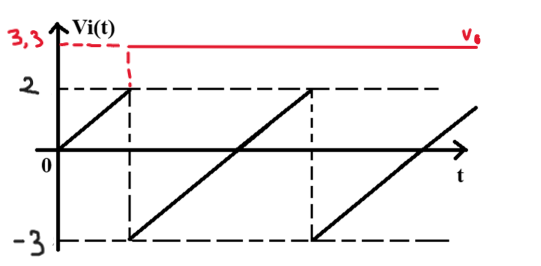
\includegraphics[scale=1]{image/C13_a_BT.png}
\end{figure}

\begin{figure}[H]
    \centering
    \begin{subfigure}[b]{0.48\textwidth}
        \centering
        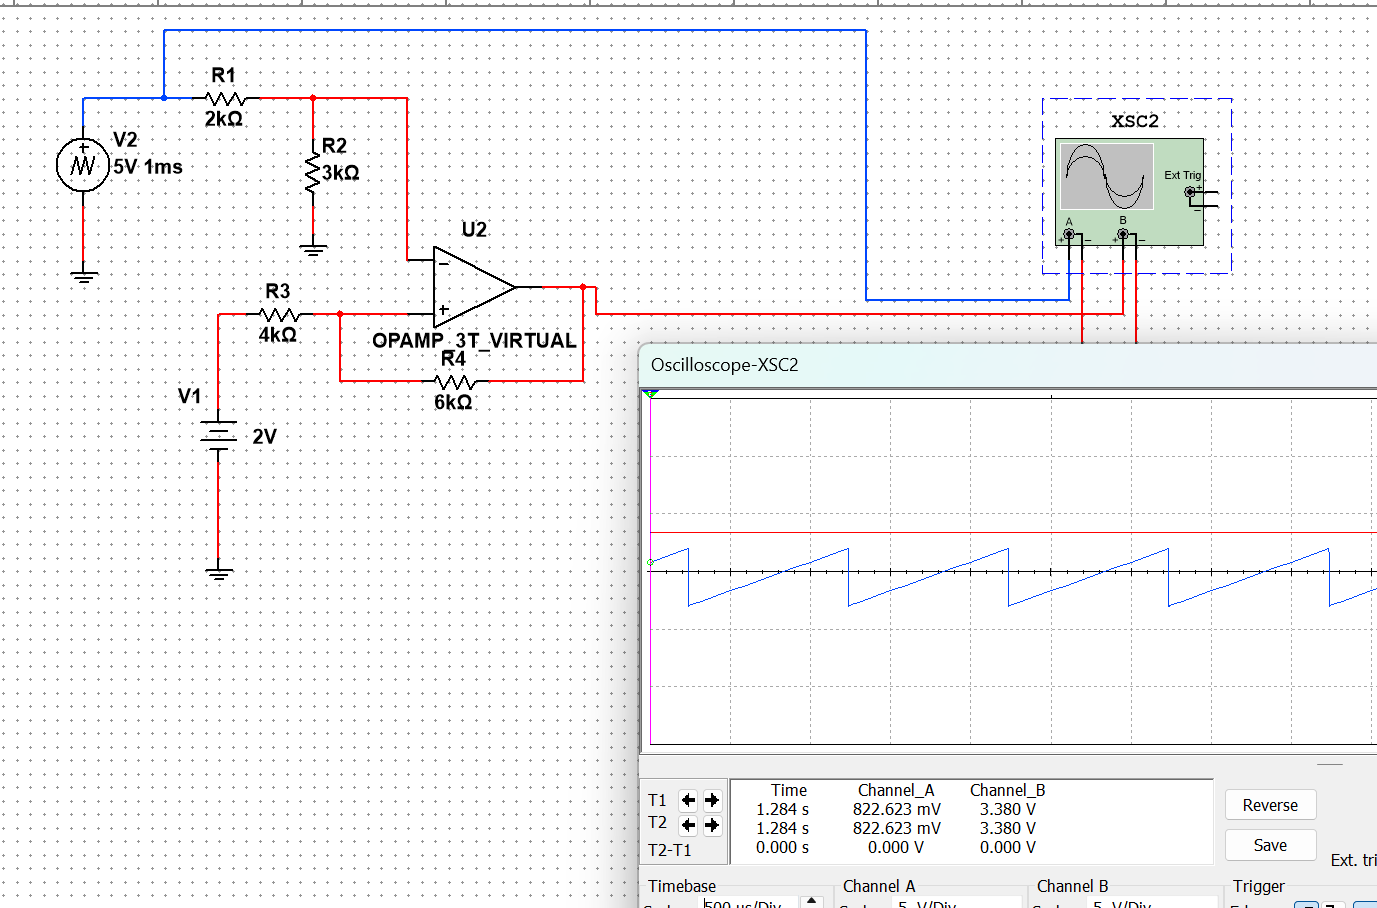
\includegraphics[width=\textwidth]{image/C13_a.png}
        \caption*{Hình a1}
    \end{subfigure}
    \hfill
    \begin{subfigure}[b]{0.48\textwidth}
        \centering
        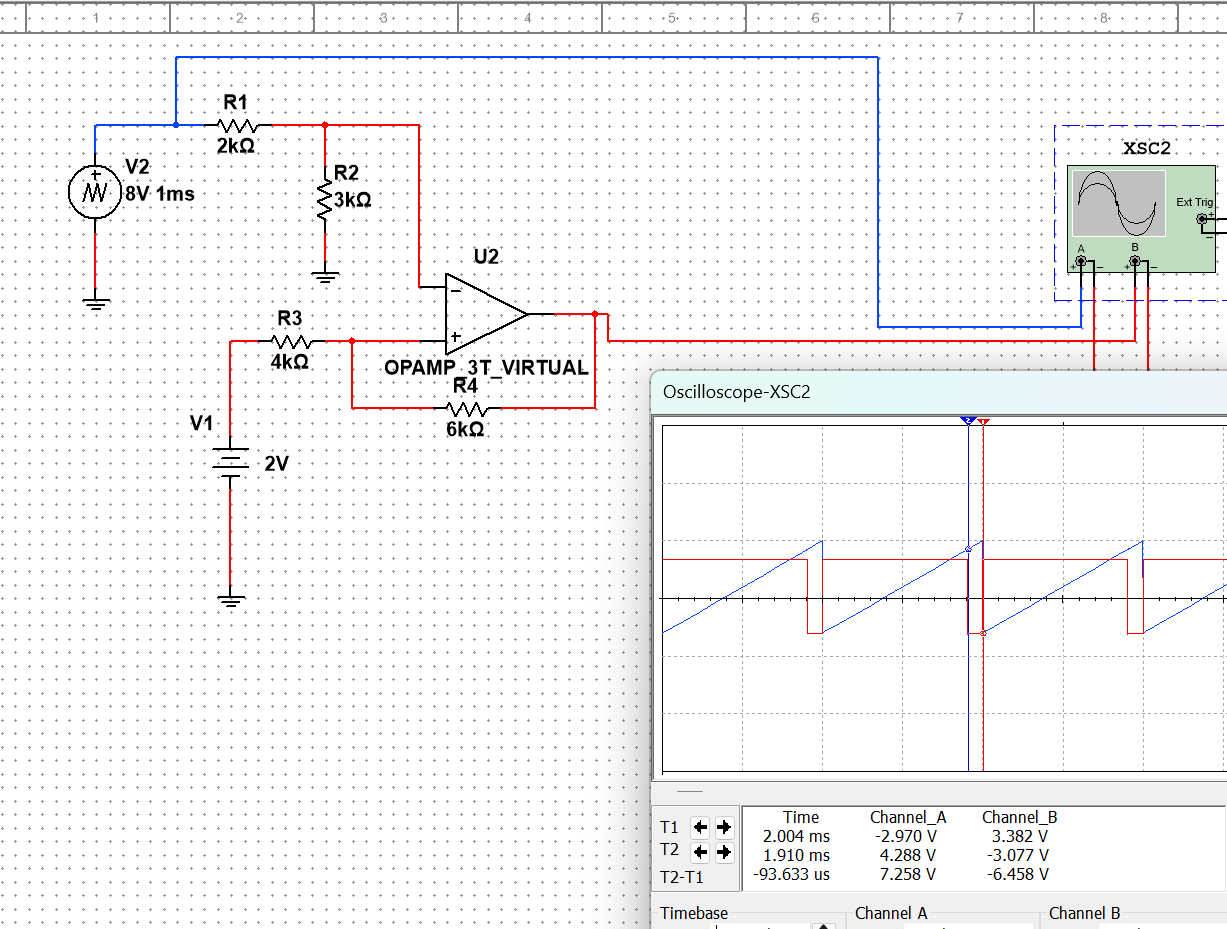
\includegraphics[width=\textwidth]{image/C13_a_1.png}
        \caption*{Hình a2}
    \end{subfigure}
\end{figure}

\textbf{Nhận xét:}\\
- Hình a1 mô phỏng $V_i$ theo đề bài với màu xanh, $V_o=-3.380V$ màu đỏ xấp xỉ 3.3V đúng với tính toán.\\
- Hình a2 chọn $V_i(t)$ thỏa $V_i>V_{UT}$ và $V_i<V_{LT}$ để kiểm tra lại $V_{UT}=4.288V$ và $V_{LT}=-2.970V$. 
Theo kết quả mô phỏng được có thể thấy $V_{UT}$ xấp xỉ 4.2V, còn $V_{LT}$ do độ dốc lớn nên không thể đo chính xác được.\\

b. Giả sử OPAMP lý tưởng:\\
Ta có:
\[
\left\{
\begin{aligned}
V^- &= \dfrac{R_2}{R_1+R_2}V_i \\
V^+ &= \dfrac{\dfrac{V_1}{R_3} + \dfrac{V_o}{R_2}}{\dfrac{1}{R_3} + \dfrac{1}{R_4}} = \dfrac{3}{5}V_1 +\dfrac{2}{5}V_o
\end{aligned}
\right.
\]

\[
\begin{aligned}
&\text{Giả sử }& V_o = V_{OH} &\qquad\rightarrow\qquad V^+ = \dfrac{3}{5}\cdot4 + \dfrac{2}{5}\cdot3.3 \quad;\quad V^- = 0.6V_i \\
&\text{Để }& V_o = V_{OL} &\qquad\rightarrow\qquad V^+ < V^- \quad\rightarrow\quad \boxed{V_i>6.2V}\\
&\rightarrow& V_o = V_{OL} &\qquad\rightarrow\qquad V^+ = \dfrac{3}{5}\cdot4 + \dfrac{2}{5}\cdot-3 \quad;\quad V^- = 0.6V_i \\
&\text{Để }& V_o = V_{OH} &\qquad\rightarrow\qquad V^+ > V^- \quad\rightarrow\quad \boxed{V_i<2V}\\
\end{aligned}
\]\\
Tại t=0 đến khi $V_i(t)=0$ nằm trong khoảng Deadband của OPAMP. Vì thế tùy vào trạng thái ban đầu sẽ cho ra ngõ ra khác nhau.
Sau khi $V_i(t)<0$ thì $V_o = V_{OH}$ và $V_i$ luôn bé hơn 6.2V nên không thể cho $V_o=V_{OL}$. Vì thế nên $V_o$ từ đó luôn bằng $V_{OH}$
\begin{figure}[H]
	\centering
	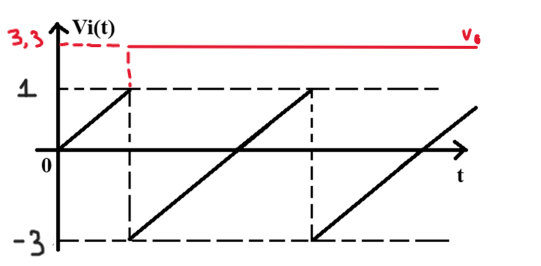
\includegraphics[scale=1]{image/C13_b_BT.png}
\end{figure}

\begin{figure}[H]
    \centering
    \begin{subfigure}[b]{0.48\textwidth}
        \centering
        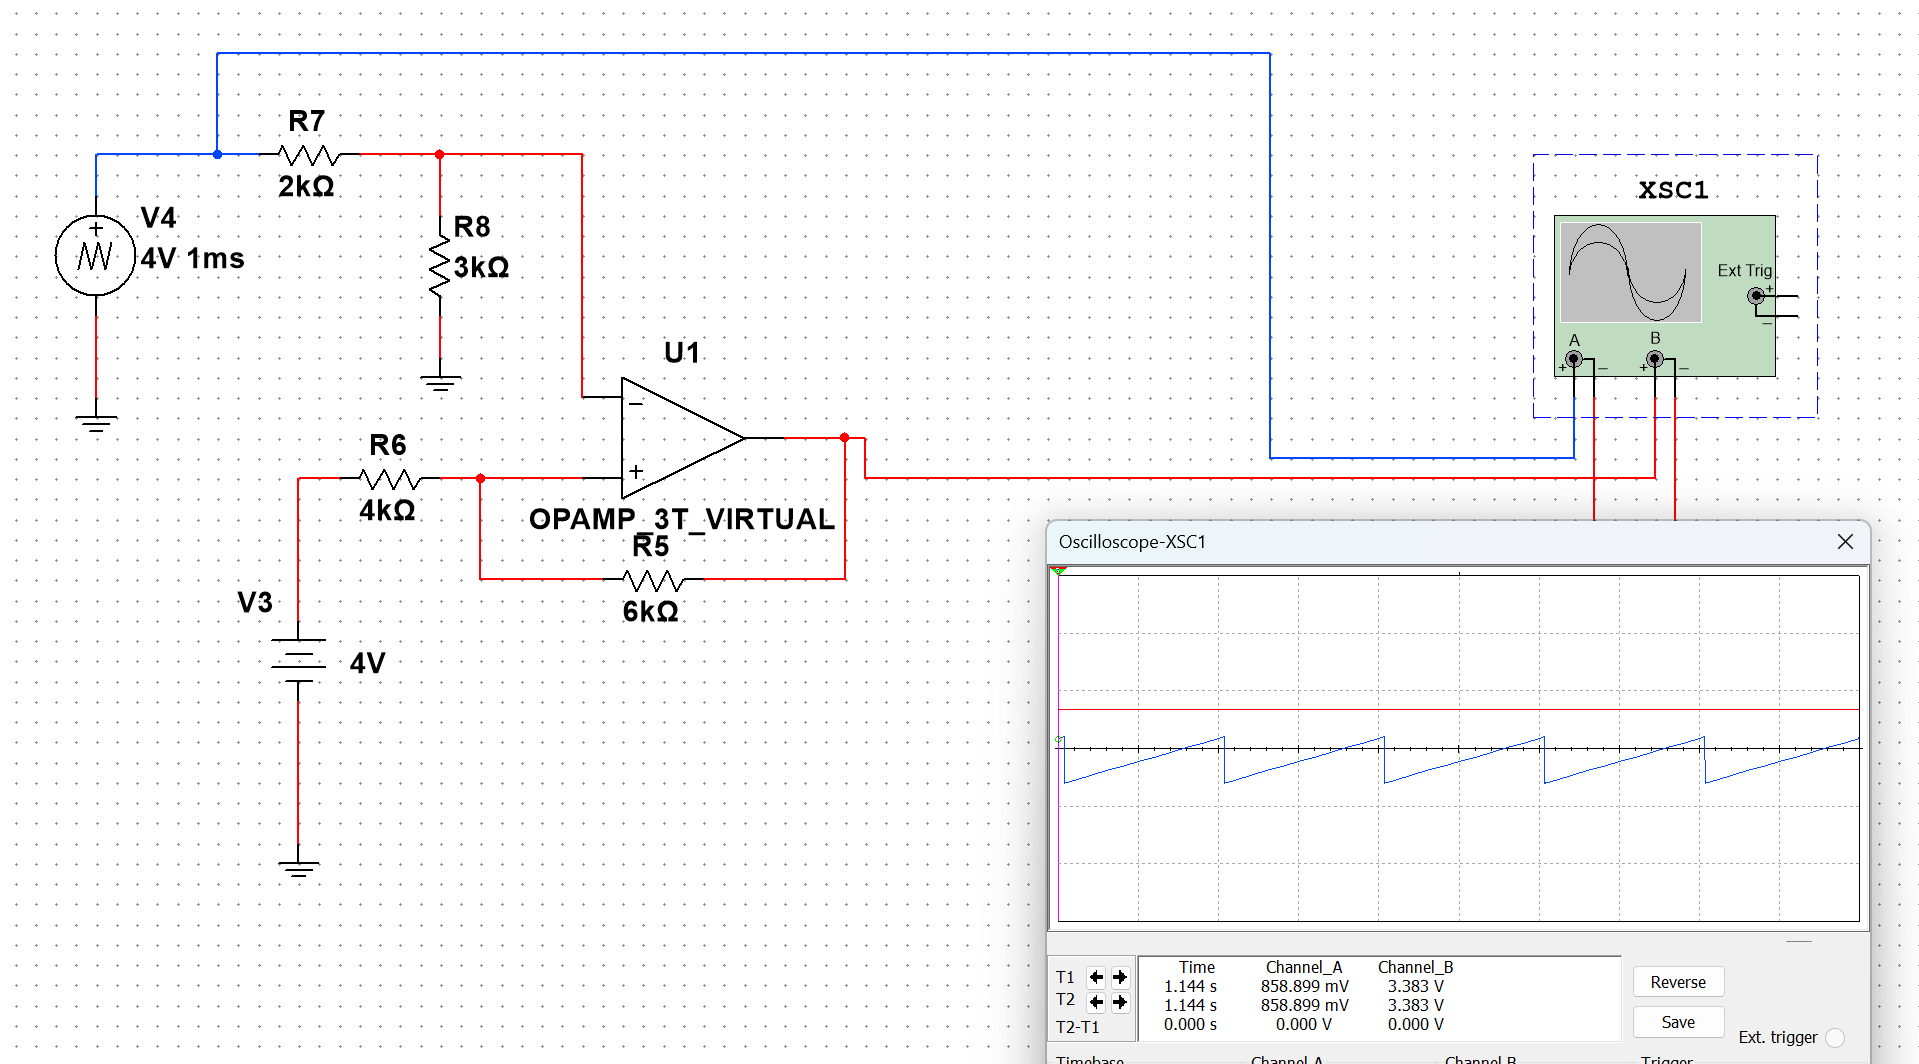
\includegraphics[width=\textwidth]{image/C13_b.png}
        \caption*{Hình b1}
    \end{subfigure}
    \hfill
    \begin{subfigure}[b]{0.48\textwidth}
        \centering
        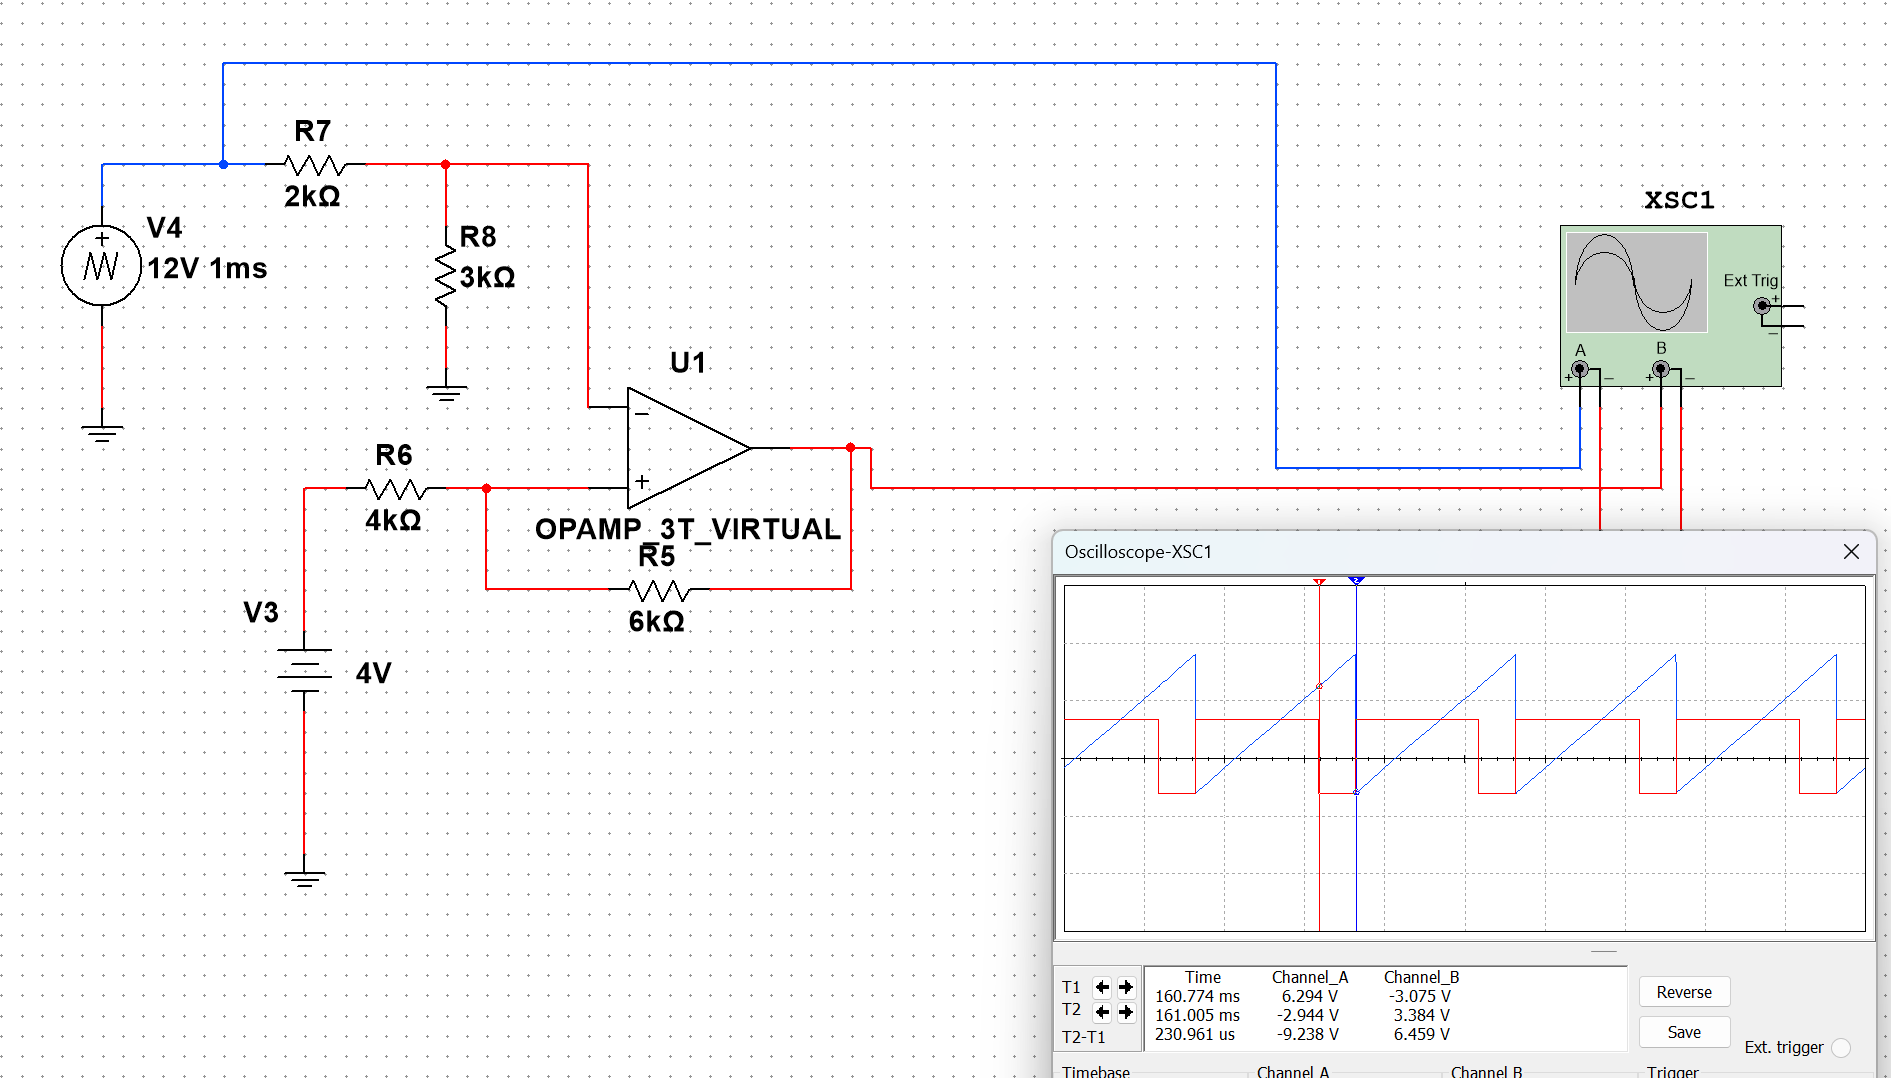
\includegraphics[width=\textwidth]{image/C13_b_1.png}
        \caption*{Hình b2}
    \end{subfigure}
\end{figure}

\textbf{Nhận xét:}\\
- Hình a1 mô phỏng $V_i$ theo đề bài với màu xanh, $V_o=-3.383V$ màu đỏ xấp xỉ 3.3V đúng với tính toán.\\
- Hình a2 chọn $V_i(t)$ thỏa $V_i>V_{UT}$ và $V_i<V_{LT}$ để kiểm tra lại $V_{UT}=6.294V$ và $V_{LT}=-2.944V$. 
Theo kết quả mô phỏng được có thể thấy $V_{UT}$ xấp xỉ 6.2V, còn $V_{LT}$ do độ dốc lớn nên không thể đo chính xác được.\\
